\section{Makahiki}
The feature set of WattDepot creates attractive infrastructure for management of energy data, but research suggests that effective participation of consumers in a next generation smart grid requires more than simple feedback to consumers about their consumption, particularly given the passive nature of their involvement for the past 100 years.

The second component of our open source software stack, Makahiki, represents research intended to create synergy between the need to create knowledge and engagement regarding energy and the ability of so-called ``serious game'' techniques and energy feedback to create participation and engagement \cite{Deterding2011mt,darby-review-2006,Faruqui09,petersen-dorm-energy-reduction}. In Makahiki, online game mechanics are employed with the goal of affecting real-world energy behaviors.  The ultimate goal is to not just affect energy behaviors during the course of the game, but to produce long lasting, sustained change in energy behaviors and outlooks by participants. Figure \ref{fig:makahiki-architecture} illustrates the architecture of Makahiki.

\begin{figure}
\begin{center}
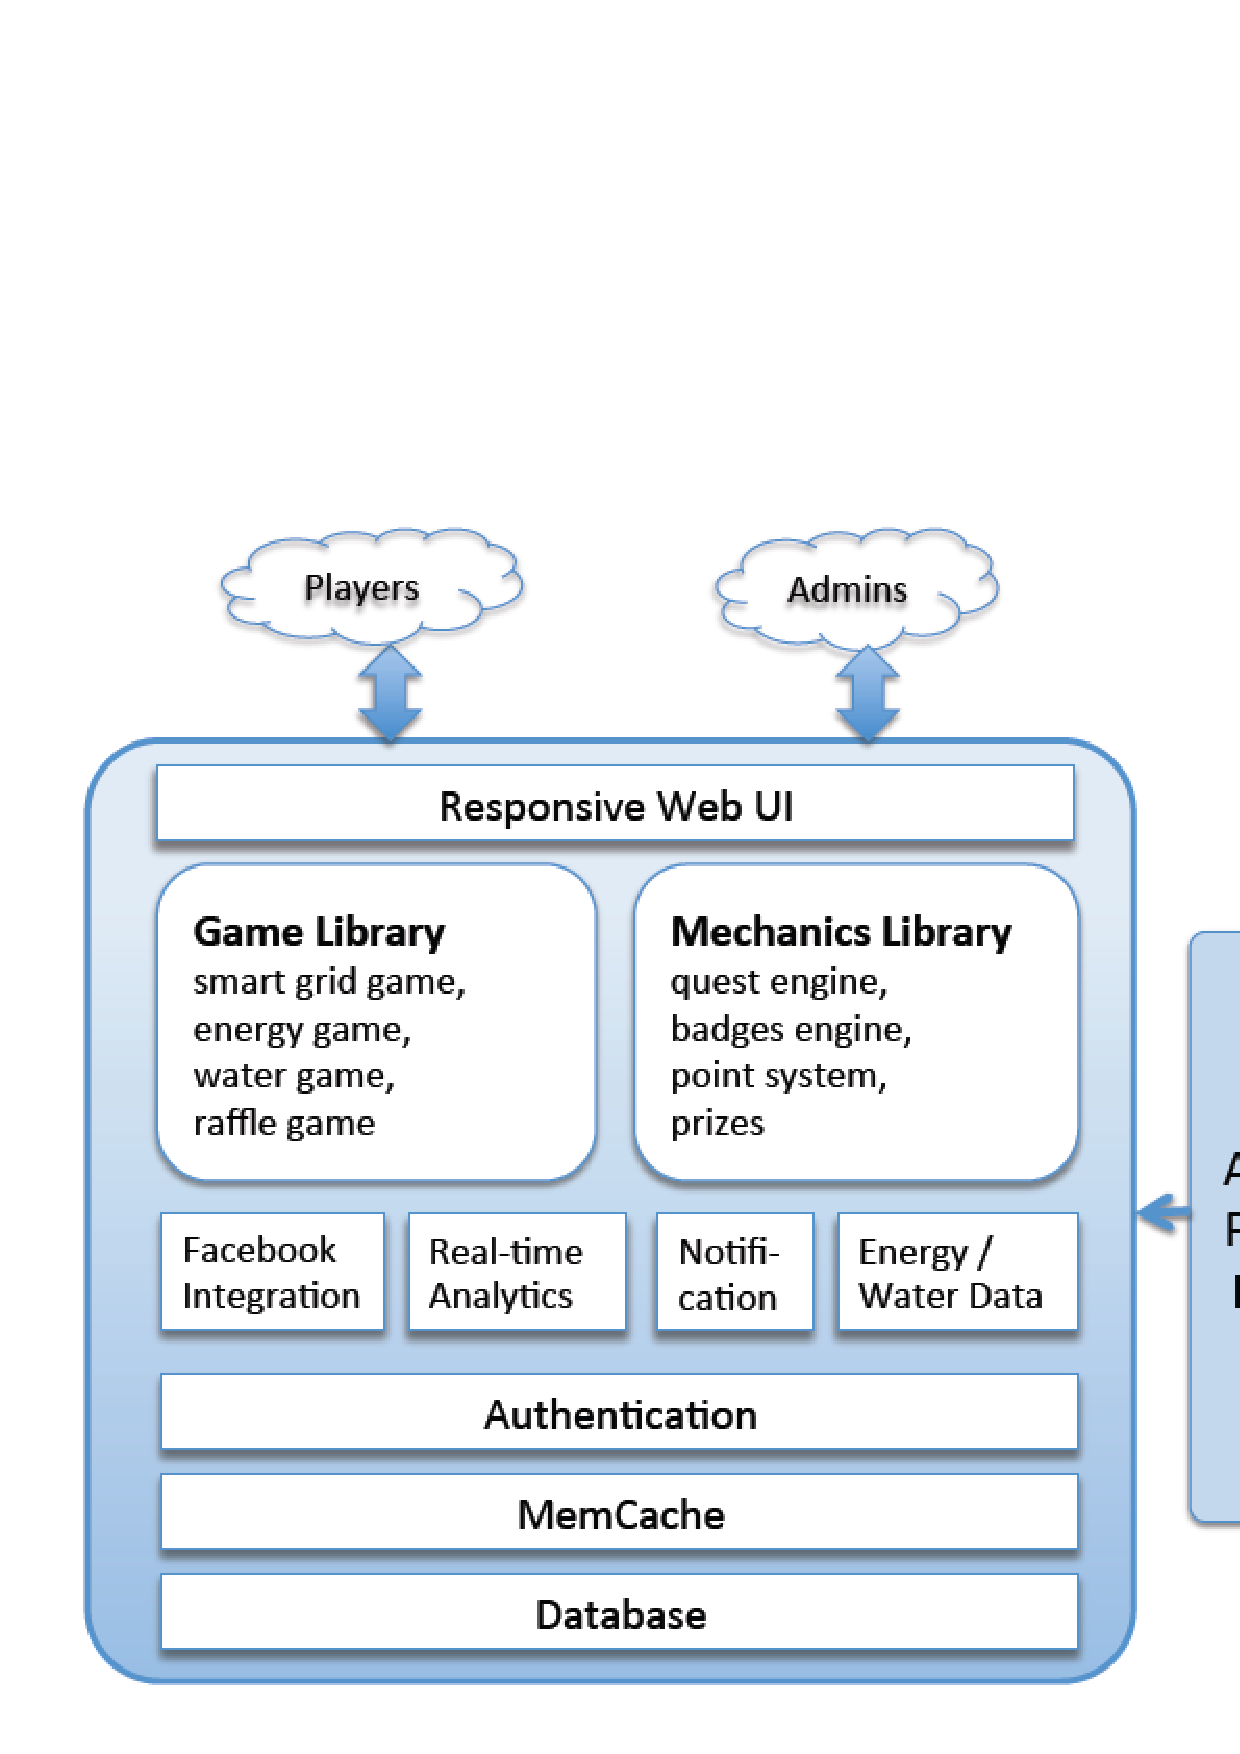
\epsfig{file=makahiki-system-architecture, width=3in}
\end{center}
\caption{Architecture of Makahiki}
\label{fig:makahiki-architecture}
\end{figure}

Makahiki consists of a configurable game engine that can be customized to the needs of different organizations.  It includes a library of pre-built game ``widgets'' that implement a variety of game mechanics.  Using the widgets, an organization can create a custom energy challenge in which players can compete individually and/or in teams to earn the most points by reducing their energy consumption as well as by learning about energy concepts in general.  The next sections present some of the most important widgets in Makahiki.

\subsection{Smart Grid Game}

The {\em Smart Grid Game widget} shown in Figure \ref{fig:SmartGrid}, is the primary place players go to learn about energy issues and earn points. Actions are organized into a grid of squares (hence the name ``Smart Grid'') and organized by category columns. The grid contains four different types of actions: activities, commitments, events, and excursions.

\begin{figure}[th]
  \center
  \includegraphics[width=0.4\textwidth]{smart-grid.eps}
  \caption{\em \small Smart Grid Game widget}
  \label{fig:SmartGrid}
\end{figure}

{\em Activities} are the most basic task available in the Smart Grid. In order to get points for an activity, a player will have to provide a response to the administrators. These responses can be a short textual answer or an uploaded picture. Administrators access a special admin section of the web application to approve or deny submissions. If a submission is approved, the player will receive the points for their submission. Otherwise, a player will be sent a website notification informing them that their submission was not approved, and a textual description by an administrator of why it was rejected. The player can change and resubmit their response and still earn the full point value for that task.

{\em Commitments} are pledges that the player will do something sustainable for a period of five days. Examples include: reducing shower time, taking the stairs, and turning off the lights when leaving a room. Because these commitments are not verifiable, they are worth fewer points than activities. Furthermore, a player can only have up to five active commitments at any given time. After the five day period is up, the player can then declare that they completed the commitment and immediately earn their points. They can then sign up for another commitment, including the one they just completed.

{\em Events and excursions} are tied to real world activities. Events are held on campus while excursions take place off campus. Seating is limited, so players are asked to sign up for events they wish to attend. Players that do so are provided with a 2 point signup bonus. Players can also set up a reminder that is sent to their email and/or their mobile phone before the event takes place. At the event, an administrator will hand out attendance codes printed on slips of paper that can be entered on the website. These attendance codes are generated by Makahiki and can only be used once. To discourage players from signing up and not attending, a 2 point penalty is assessed to players who do not submit an attendance code. If the player submits an attendance code for the event after receiving this penalty, the penalty is reversed.

Not all of the tasks in the Smart Grid Game are necessarily available at
the start of the game. We implemented a set of predicates that can be used to determine if a task is locked or unlocked for a player. These predicates include: completed a certain number of tasks within a category, completed all tasks within a category, completed certain tasks, and time-based unlocking (available after a certain date).

These predicates are implemented using a limited subset of Python and can
be changed within the Django admin interface. Competition designers can use
logical operators to combine any of these functions in order to organize
the players' path through the Smart Grid Game.

\subsection{Power Meter}

A fundamental requirement for enabling more active participation by consumers in the smart grid is feedback regarding their energy usage.  One of the most simple mechanisms provided by Makahiki for this purpose is the Power Meter widget, illustrated in Figure \ref{fig:PowerMeter}.

\begin{figure}[th]
  \center
  
\includegraphics[width=0.4\textwidth]{power-meter.eps}
  \caption{\em \small Power Meter widget}
  \label{fig:PowerMeter}
\end{figure}

The Power Meter widget provides basic feedback on energy consumption via a display of the team's power consumption, updated every few seconds.  The visualization can normalized using baseline values so that when the needle is pointing straight up, the power consumption is average for that team during that specific hour of that specific day of the week.  Thus, if the needle leans left toward the green side, the team's power consumption at that moment in time is below average, while if the needle leans right toward the red side, the team's power consumption at that moment in time is above average.  

The Power Meter widget obtains its values by querying the WattDepot system for the latest power data consumed by the associated team.  The use of WattDepot, rather than directly querying the meter(s), simplifies the widget design significantly.  First, the physical meters can vary significantly in the protocol implemented to obtain current power consumption.   These protocol variations are handled by the WattDepot sensors, so this widget can simply query the WattDepot server using a simple single HTTP request that is independent of the physical meter characteristics.  Second, the power consumed by a team might be measured by one or multiple meters.  Again, the WattDepot virtual source capability means that this physical difference can be abstracted away by WattDepot, enabling the widget to obtain the aggregate power for the team through a single HTTP request. 

The Power Meter widget is a useful, though simple mechanism for energy feedback that uses the WattDepot+Makahiki stack.   The next section presents a more sophisticated mechanism called the Daily Energy Goal Game.

\subsection{Daily Energy Goal Game}

The {\em Daily Energy Goal Game widget} provides a way for players to earn points by reducing their current consumption from a baseline. Both the baseline data and the current consumption is typically provided by API calls from Makahiki to an underlying WattDepot server.
Figure \ref{fig:DailyEnergyGoal} illustrates this widget.

\begin{figure}[th]
  \center
  \includegraphics[width=0.4\textwidth]{daily-energy-goal-game.eps}
  \caption{\em \small Daily Energy Goal Game widget}
  \label{fig:DailyEnergyGoal}
\end{figure}

The goal for each team is typically a percent reduction from their baseline usage of the previous two weeks. When a player goes to the energy page of Makahiki, they can view their team's current progress toward their daily energy goal. Near the end of the day, Makahiki checks the energy data from Wattdepot to see if a floor reached their goal. If the floor did reach their goal, each member of the floor that is participating in the game receives 20 points. The energy goal game provides a link between the energy conservation competition and the point competition.

The Daily Energy Goal display shows both their current progress and their goal so far for two reasons. First, everyone will be under their actual energy goal for most of the day, so this display would not be very useful. Second, we have noticed that the students in the residence halls use more energy at night rather than during the day. Thus, it is easy to be under for most of the day and then jump over the goal at the very end. Displaying their progress toward the goal so far provides a pace for players to follow.

\subsection{Raffle Game}

The {\em Raffle Game widget} provides a way to incentivize participation from all individuals, even those who are not in the running for a top prize. For every 25 points a player earns, they receive one virtual raffle ticket. Players can dynamically allocate their tickets to any raffle prizes they are interested in at any time, up to the end of the raffle.  Figure \ref{fig:RaffleGame} shows an example of the Raffle Game. 


\begin{figure}[th]
  \center
  \includegraphics[width=0.4\textwidth]{raffle-small.eps}
  \caption{\em \small Raffle Game widget}
  \label{fig:RaffleGame}
\end{figure}

Players can dynamically allocate their tickets to any raffle prizes they are interested in at any time, up to the end of the raffle. Each round of the competition has its own set of raffle prizes and any unused raffle tickets carry over to the next round. Raffle tickets are independent from a player's score; allocating a raffle ticket does not affect their rank. 

\subsection{Social and Referral Bonuses}

The {\em Social and Referral Bonus widgets} provide game mechanics that help encourage participation by providing additional points to players who participate in activities with other players and/or facilitate the entry of new players into an energy challenge.

The social bonus is an administrator option when a task is created in the Smart Grid Game. It awards extra points if the player has done the task with someone else. Examples of tasks with social bonus include attending an event, recording a song related to energy, or measuring a shower water flow rate. When a player submits a response for a task with a social bonus, the player can provide the email address of the person who jointly completed the task. Once the other player completes the task, the social bonus is awarded. Social bonuses are not bi-directional; if the second player doesn't provide the first player's email address, only the first player will get the social bonus.

Players are led through a setup process when logging into Makahiki for the first time. One of the steps in this process is the referral bonus. If a player was referred by another player in the system, they can use this step to input their email address. Once the new player earns 30 points in the competition, both players are awarded a referral bonus of 10 points. Typically, going through the setup process gives you 25 points, so we wanted to encourage the new player to at least complete one additional task in order to get the referral bonus.

\subsection{Quest Engine}

One challenge we faced when designing Makahiki was providing adequate help to the player. The game needed to be intuitive, even if a new player coming to Makahiki has not participated in an energy competition. Unlike many web applications, such as webmail, game players generally do not know in advance what specific tasks they wish to accomplish. In an effort to provide a player with guidance through Makahiki after the setup process, we implemented the Quest Engine. Quests are used to guide the player through the various workflows of the site, like completing a task, signing up for an event, or allocating a raffle ticket. These quests can be created in the admin interface. They also use a set of predicates to determine unlock and completion conditions. These predicates are: participating in a task or type of task, completed a task or type of task, has a certain number of points (in a round or overall), completed a certain number of tasks in a category or of a given type, awarded a badge, wrote a post on their floor wall, and added a picture to their profile.

\subsection{Game Analytics}

Makahiki is designed to support energy challenges involving hundreds or thousands of users lasting weeks or months.  In these circumstances, effective use of the technology requires the ability to understand the state of the game, such as: Who is using it? What are they doing? What is the player response to activities, commitments, excursions, and events?   Such state information is important for planning purposes, such as assessing the transportation needs for an upcoming excursion by seeing how many players signed up.   It can also be used for making in-game changes to game analytics, such as changing the point values associated with activities to encourage or discourage participation.  It can also help identify breakdowns in game play, such as significant numbers of unallocated raffle tickets indicating that users do not understand the nature of that game mechanic.  

To address these needs and others, Makahiki includes a variety of widgets that work together to provide high level game play state to the administrators of a challenge. Figure \ref{fig:status} shows an example of two game analytic widgets.

\begin{figure}[t!]
  \center
  \includegraphics[width=0.4\textwidth]{status.eps}
  \caption{Game analytic widgets: User Stats and Energy Goal Status}
  \label{fig:status}
\end{figure}

The top widget, User Stats, shows trends in the total number of players, the total number of new users, and the total number of players visiting the site each day.  The bottom widget provides information on the ability of teams to achieve their daily energy goal each day and over time.  

We have now introduced the primary components of our software stack, WattDepot and Makahiki.  The next section presents our experiences and lessons learned so far. 



